\documentclass[12pt, oneside, a4paper]{article}
\usepackage[utf8]{inputenc}
\usepackage[T1]{fontenc}
\usepackage[english]{babel}
\usepackage[babel,german=quotes]{csquotes}

\usepackage{graphicx}
\usepackage{float}
\usepackage[normalem]{ulem}
\usepackage{amssymb}

\usepackage[backend=biber, style=ieee]{biblatex}
% \addbibresource{paper.bib}



\usepackage{listings}
\usepackage{rotating}
\usepackage{pdflscape}
\usepackage{adjustbox}

\usepackage[left=2.5cm,right=2.5cm,top=2.5cm,bottom=2.5cm]{geometry}
\linespread{1.5}

% höly fucking shit what the fuck
% so just doing backref does not work, but backref=true works
% fyi this makes \ref commands clickable
\usepackage[hidelinks, backref=true]{hyperref} 
\usepackage[nonumberlist,automake=immediate,toc]{glossaries}

\makeglossaries
\newcommand{\projektname}{Modellierung eines Ticketsystems}
\newcommand{\autor}{Emil Schläger}
\newcommand{\matrikelnummer}{2988631}
\newcommand{\set}[1]{\{#1\}} % HOLY SHIT LATEX WHAT THE FUCK ARE YOU DOING
\newcommand{\relation}[2]{$$\text{{#1}: } \set{[{#2}]}$$}

%% Define custom commands END!

\begin{document}
	\pagenumbering{gobble}
	% Deckblatt
	\begin{center}
		% \href{https://www.intension.de/}{\includegraphics[width=6cm]{images/intension}}\hfill\href{https://www.dhbw-stuttgart.de}{\includegraphics[width=4cm]{images/dhbw}}\\
		\large
		\vspace{3cm}
		\textbf{Semesterprojekt Datenbanken}:\\
		\projektname{}
	\end{center}
	\vfill
	\textbf{Name:}\hfill \autor{}\\
	% \textbf{Matrikelnummer}\hfill \matrikelnummer{}
	\textbf{Kurs:}\hfill INF23B
	

	\newpage
	\tableofcontents
	\newpage
	\listoffigures
	
	
	\newpage
	\pagenumbering{arabic}
	\section{Anforderungsanalyse}
Es soll eine Ticketplattform entstehen, die es Veranstaltern und Künstlern ermöglicht, Events zu planen und Tickets an Kunden zu verkaufen.\\
Um die Plattform nutzen zu können, muss man sich als User anmelden. Für eine Konto müssen der volle Name, eine Email-Adresse, ein Passwort und eine Kontonummer hinterlegt werden. Angabe einer Telefonnummer für Zwei-Faktor Authentifizierung ist optional. Als User kann man nun Tickets zu Events kaufen. Jedes Ticket besitzt einen Preis, sowie eine Kategorisierung, ob es ein Sitz- oder Stehplatzticket ist. Ist es ein Sitzplatzticket, muss noch die Sitznummer hinterlegt werden. Dabei darf für ein Event selbstverständlich nicht mehrfach derselbe Sitz gebucht werden. Für das jeweilige Event muss gespeichert werden, an welchem Tag es stattfindet, sowie um welche Uhrzeit es anfängt. Es kann auch hinterlegt werden, um wie viel Uhr Einlass ist. Auch findet jedes Event in genau einer Venue statt. Für diese ist jeweils ihr Name, ihre Adresse und ihre Kapazität hinterlegt. Die Kapazität ist hierbei aufgeteilt in die Anzahl an möglichen Steh- und möglichen Sitzplätzen.\\ 
Ein Event ist immer ein Teil einer Tour. Jede Tour ist von einem Veranstalter organisiert, und dementsprechend auch auf der Plattform verwaltet. Z.B. können einzelne Events in größere Venues verlegt werden, wenn das Event ausverkauft ist, aber noch Nachfrage existiert. Zu jeder Tour muss nur der Name gespeichert werden; der Zeitrahmen der Tour errechnet sich durch die Daten des frühesten und spätesten Events der Tour.\\
Auf einer Tour spielt immer mindestens ein Künstler. Oft bringt der Künstler aber Vorbands mit. In diesem Fall ist wichtig zu speichern, in welcher Reihenfolge die Künstler in der Tour spielen. Der Hauptkünstler spielt dabei stets als letztes. Jeder Künstler hat einen Namen und gehört einem Genre an.  Ein Künstler spielt auf jedem Event einer Tour immer dieselbe Setlist. Die Plattform gibt Künstlern die Möglichkeit, diese Setlist auf der Plattform für ihre Fans zu veröffentlichen. Eine Setlist besteht aus mehreren Songs, die wiederum Teil eines Albums sind. Auch diese sind für User der Plattform auf den Profilen der Künstler einzusehen. Ein Album wird immer von einem Label veröffentlicht, auch Künstler sind immer bei einem Plattenlabel unter Vertrag. Für jedes Label muss sein Name, sowie die Adresse seines Hauptsitzes gespeichert werden. Für den Vertrag zwischen Label und Künstler muss auch ein Ablaufdatum gespeichert werden.\\
Die Plattform soll auch die Finanzen einer Tour verwalten können, da die Bezahlung der Tickets bei der Plattform landet.  Organisiert also ein Veranstalter eine Tour für einen Künstler, entsteht dabei ein weiterer Vertrag, der vereinbart, wie viel Prozent der Umsätze der Tour an den Veranstalter gehen. Der Umsatz einer Tour errechnet sich ganz einfach aus der Summe der Preise aller verkauften Tickets. Auch die Plattenlabel verdienen an den Tickets mit. Dieser Festbetrag errechnet sich wie folgt: Bei Veröffentlichung eines Albums $A$ über Label $L$ wird ein Betrag festgelegt, der an das Label gezahlt wird, jedes mal wenn der Künstler einen Song $s \in A$ spielt. Am Ende einer Tour kann also mithilfe der Setlist der Künstler und der Anzahl an Events ausgerechnet werden, wie viel an das Label gezahlt werden muss.\\
Da Künstler, Veranstalter und Label jeweils Zugang auf die Plattform haben müssen, um die für sie relevanten Daten zu verwalten, muss jedem indivuduellen Künstler, Veranstalter oder label ein User Account zugeordnet werden. Damit die Plattform entscheiden kann, welche Zugriffsrechte ein einzelner User hat, wird jedem Account eine entsprechende Rolle zugeordnet.

\newpage
\section{Konzeptioneller Entwurf}
\vspace*{\fill}
\begin{adjustbox}{angle=90,center,caption=Entity Relationship Model,nofloat=figure}
	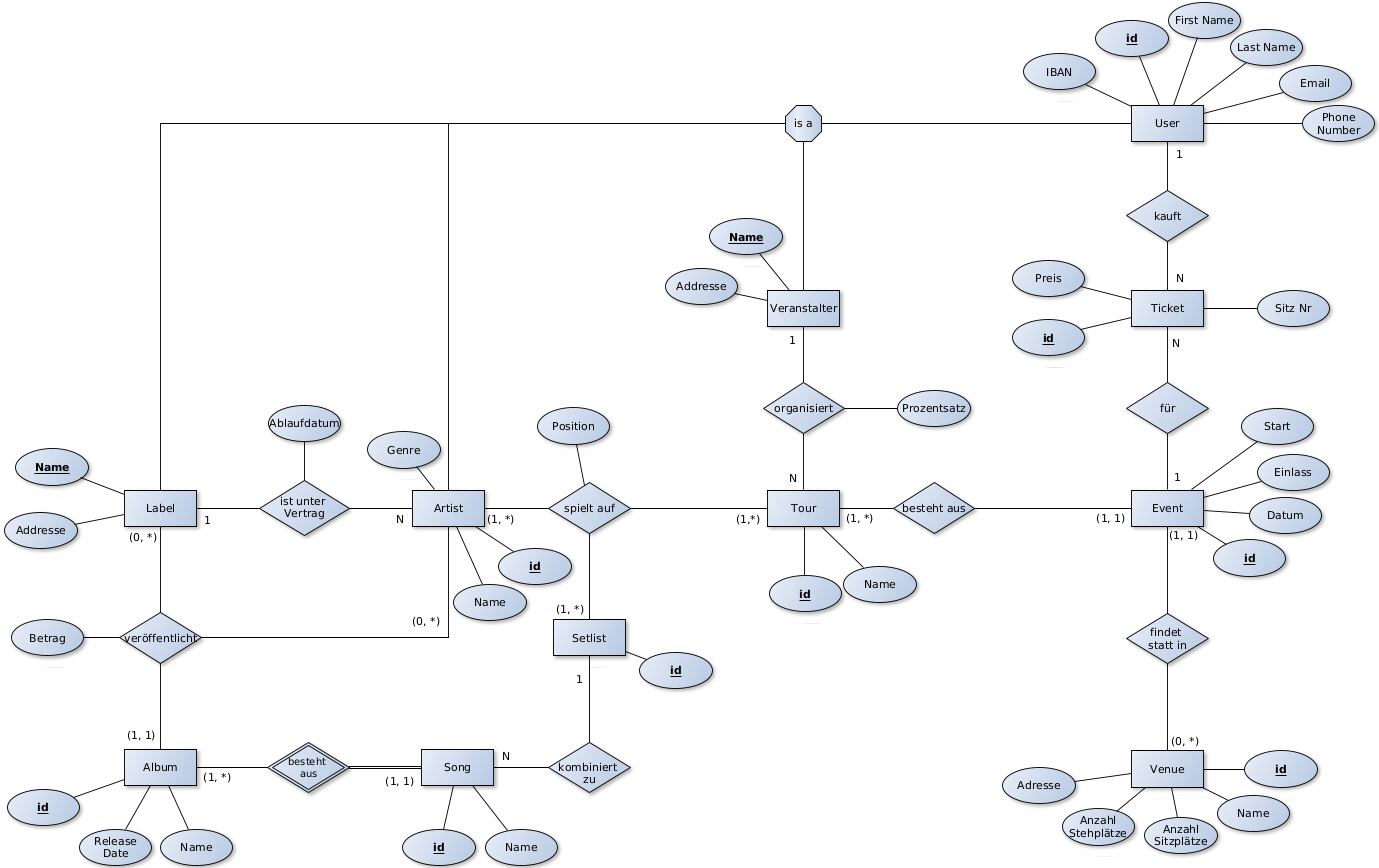
\includegraphics[width=1.4\textwidth]{img/erm_corrected_again.png}
	\label{fig:erm}
\end{adjustbox}





\newpage
\section{Logischer Entwurf}
\subsection{Relationales Modell}

\relation{User}{{\underline{User\_ID}},\ First\_Name,\ Last\_Name,\ Email,\ Phone\_Number}
\relation{Ticket}{\underline{Ticket\_Nr},\ Price,\ Seat\_Nr,\ \dashuline{User\_ID},\ \dashuline{Event\_ID}}
\relation{Event}{\underline{Event\_ID},\ Begin,\ Doors,\ Date,\ \dashuline{Venue\_ID}, \dashuline{Tour\_ID}}
\relation{Venue}{\underline{Venue\_ID},\ Name,\ \dashuline{Address},\ Capacity\_Standing,\ Capacity\_Seated}
\relation{Tour}{\underline{Tour\_ID},\ Name,\ \dashuline{Organizer\_ID},\ Percentage}
\relation{Artist}{\underline{Artist\_ID},\ Name,\ Genre,\ \dashuline{Label\_Name},\ Contract\_End,\ \dashuline{User\_ID}}
\relation{Setlist}{\underline{Setlist\_ID}}
\relation{Plays\_In}{\dashuline{\underline{Artist\_ID}},\ \dashuline{\underline{Tour\_ID}}, \dashuline{\underline{Setlist\_ID}},\ Position}
\relation{Song}{\underline{Song\_ID},\ \dashuline{\underline{Album\_ID}},\ Name,\ \dashuline{Setlist\_ID}}
\relation{Album}{\underline{Album\_ID},\ Name,\ Released, \dashuline{Label\_Name}}
\relation{Label}{\underline{Name},\ \dashuline{Address},\ \dashuline{User\_ID}}
\relation{Releases}{\dashuline{\underline{Artist\_ID}},\ \dashuline{\underline{Album\_ID}}, \dashuline{{Label\_Name}}, Label\_Fee}
\relation{Organizer}{\underline{Name},\ \dashuline{Address},\ \dashuline{User\_ID}}
\relation{Address}{\underline{Address\_ID},\ Country,\ City,\ Postal\_Code,\ Street,\ House\_Number}


\subsection{Exemplarisches Prüfen auf 3NF}
% Die Relation \textit{Address} ist aufgrund der Normalisierung in 3NF neu entstanden. Hier wird formal aufgezeigt, wie diese Notwendigkeit zustande kommt.

% Im ERM (\ref{fig:erm}) ist zu sehen,dass die Entität \textit{Venue} ein Attribut \textit{Adresse} besitzt. Ein solches Attribut ist aber nicht atomar, da sich eine Adresse aus mehreren Bestandteilen zusammensetzt. Da als Resultat eine Relation mit diesem Attribut nicht einmal in der 1. Normalform wäre, muss hier normalisiert werden.

% \subsubsection{1NF}
% Um \textit{Venue} in 1NF zu bringen, muss das Attribut \textit{Adresse} in seine Bestandteile zerlegt werden. Damit sieht die Relation \textit{Venue} nun wie folgt aus:
% \begin{align*}
% 	\text{Venue: } \set{\underline{Venue\_ID},\ Name,\ Capacity\_Standing,\ Capacity\_Seated,\\
% 	Country,\ City,\ Postal\_Code,\ Street,\ House\_Number}
% \end{align*}

% \subsubsection{2NF}


Hier wird am Beispiel der Relation \textit{Venue} gezeigt, dass diese in der 3. Normalform ist.
Hierfür müssen zunächst 1NF und 2NF geprüft werden:
\begin{itemize}
	\item 1NF: Alle Attribute sind so konzipiert, dass sie nur einen wert enthalten, also atomar sind. Dadurch ist die Relation in 1NF.
	\item 2NF: Der Primärschlüssel der Relation, $\set{Venue\_ID}$, enthält nur ein Element. Dadurch kann es keine funktionalen Abhängigkeiten von einem Teil des Schlüssels geben. Dadurch ist die Relation in 2NF.
\end{itemize}

Um zu prüfen, ob die Relation in 3NF ist, müssen zuerst alle existierenden funktionalen Abhängigkeiten innerhalb der Relation bestimmt werden:
$$F = \begin{cases}Venue\_ID \rightarrow [Venue] \\ Name,\ Address \rightarrow [Venue]\end{cases}$$


Dadurch ergeben sich zwei Schlüsselkandidaten: $\set{Venue\_ID}$ und \smallskip $\set{Name,\ Address}$. Anhand der folgenden Tabelle werden alle funktionalen Abhängigkeiten der Form $$X \rightarrow \alpha$$ untersucht:

\begin{table}[H]
\centering
\begin{tabular}{|c|c|c|c|}
\hline
X & $\alpha$ & $X$ ist Superschlüssel & $\alpha$ ist prim \\ \hline
Venue\_ID & Name & \checkmark & \text{\sffamily X} \\ \hline
 & Address & \checkmark & \checkmark \\ \hline
 & Name & \checkmark & \checkmark  \\ \hline
 & Capacity\_Seated & \checkmark & \text{\sffamily X} \\ \hline
 & Capacity\_Standing & \checkmark & \text{\sffamily X} \\ \hline
Name, Address & Venue\_ID & \checkmark & \checkmark \\ \hline
 & Capacity\_Seated & \checkmark & \text{\sffamily X} \\ \hline
 & Capacity\_Standing & \checkmark & \text{\sffamily X} \\ \hline
\end{tabular}
\caption{3NF Prüfung für Ticket}
\label{tab:example}
\end{table}

Da für jede Funktionale Abhhängigkeit $f \in F$ gilt, dass die Domäne von $f$ ein Superschlüssel ist, oder die Bildmenge ein Primattribut, ist die Relation in 3NF.

\newpage
\section{Datenbankschema}
Korrekturen, die für diesen Teil an der Modellierung vorgenommen wurden:
\begin{itemize}
	\item Beziehung "Song kombiniert zu Setlist" wurde von einer 1-N Beziehung in eine N-M Beziehung transformiert. Dies ist ein Ergebnis dessen, dass Löschregeln sonst semantisch nicht sinnvol definiert werden könnten.
\end{itemize}

\subsection{Keine Cascade Zyklen}
Hier wird gezeigt, dass es keine Zyklen aus Löschregeln gibt, die zu ungewolltem Datenverlust führen könnten. Hierfür wird in einer Tiefensuche jeder \texttt{on delete cascade} foreign key constraints überprüft, was passieren würde, wenn er ausgelöst würde. Die benutzte Darstellung ist wie folgt zu lesen: "Tabelle, in der ursprünglich gelöscht wird" $\rightarrow$ "Tabelle, in der dies zu einer Cascade führt".

\begin{enumerate}
	\item \texttt{event} $\rightarrow$ \texttt{ticket}: \texttt{ticket} wird von keiner weiteren Tabelle referenziert.
	\item \texttt{artist, tour, setlist} $\rightarrow$ \texttt{plays\_in}: \texttt{plays\_in} wird von keiner weiteren Tabelle referenziert.
	\item \texttt{setlist, song} $\rightarrow $\texttt{part\_of}: \texttt{part\_of} wird von keiner weiteren Tabele referenziert.
	\item \texttt{album} $\rightarrow$ \texttt{song}: Löschen in \texttt{song} löst ein Löschen in \texttt{part\_of} auf, welches von keiner weiteren Tabelle referenziert wird.
	\item \texttt{artist, album, music\_label} $\rightarrow$ \texttt{releases}: \texttt{releases} wird von keiner weiteren Tabelle referenziert.
\end{enumerate}

Somit existiert nirgends ein Zyklus aus Cascades, ungewolltes Verhalten kann also in dieser Hinsicht ausgeschlossen werden.

\end{document}